\section*{Problem 1}

Compute the DTFT of the following signals and sketch $X(\omega)$.

%%%%%%%%%%%%%%%%%%%%%%%%  a  %%%%%%%%%%%%%%%%%%%%%%%%%%
\begin{itemize}
\item 
$x[n] =
\left[
\begin{array}{c c c c}
 \frac{1}{4}&  \frac{1}{4}& \frac{1}{4}& \frac{1}{4}
 \end{array}
 \right]
$
\end{itemize} 

\subsection*{Solution}

Aplying the definition of (\ref{eq:c41}) we have:

\begin{equation*}
\begin{aligned}
X(\omega) &= \displaystyle\sum_{0}^{3} \frac{1}{4} e^{-j \omega n} \\
&= \frac{1}{4} [1 + e^{-jw} + e^{-2jw} + e^{-3jw}] \\
&= \frac{1}{4} e^{-j \frac{3 \omega}{2}}
		[e^{j \frac{3 \omega}{2}} + e^{-j \frac{\omega}{2}} + 
		 e^{- j \frac{\omega}{2}} + e^{-j \frac{3 \omega}{2}} ] \\
&= \frac{1}{2}  e^{-j \frac{3 \omega}{2}} [\cos(\frac{3 \omega}{2})\cos(\frac{\omega}{2})]
\end{aligned}
\end{equation*} 

The plot of the magintude $X(\omega)$ is:
\zcodemat{sources/c4p1a.m}{Plot of Magnitude}

\begin{figure}[H]
\caption{Magnitude $|X(\omega)|$}
\centering
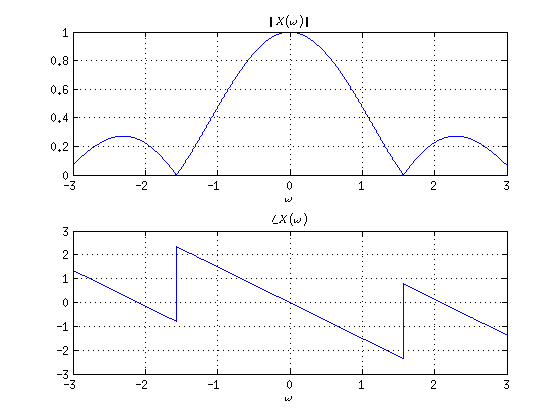
\includegraphics[width=0.6\textwidth]{figs/c4p1a.png}
\label{fig:c4p1a}
\end{figure} 

%%%%%%%%%%%%%%%%%%%%%%%%  b  %%%%%%%%%%%%%%%%%%%%%%%%%%
\begin{itemize}
\item 
$x[n] =
\left[ \begin{array}{c c c}
1 & -2 & 1
\end{array} \right] $
\end{itemize} 

\subsection*{Solution}

Aplying the definition of (\ref{eq:c41}) we have:

\begin{equation*}
\begin{aligned}
X(\omega) &= \displaystyle\sum_{0}^{2} x[n] e^{-j \omega n} \\
&= [1 - 2e^{-jw} + e^{-2jw} ] \\
&= e^{-jw} [e^{jw} - 2 + e^{-jw} ] \\
&= e^{-jw}) 2[ \cos(\omega) - 1 ] \\
&= 2e^{-jw}[ \cos(\omega) - 1 ] 
\end{aligned}
\end{equation*} 

The plot of the magintude $X(\omega)$ is:
\zcodemat{sources/c4p1b.m}{Plot of Magnitude}

\begin{figure}[H]
\caption{Magnitude $|X(\omega)|$}
\centering
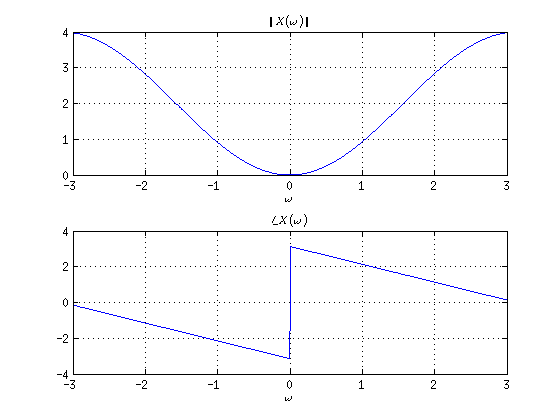
\includegraphics[width=0.6\textwidth]{figs/c4p1b.png}
\label{fig:c4p1b}
\end{figure} 

%%%%%%%%%%%%%%%%%%%%%%%%  c  %%%%%%%%%%%%%%%%%%%%%%%%%%
\begin{itemize}
\item 
$x[n] =2\big(\frac{3}{4}\big)^n u[n] $
\end{itemize} 

\subsection*{Solution}

\begin{equation*}
X(\omega) = \displaystyle\sum_{0}^{\infty} 2\big(\frac{3}{4}\big)^n e^{-j \omega n} 
\end{equation*} 

Recall that the geometric series solution is given by:

\begin{equation}
\displaystyle\sum_0^{\infty} a r^n = \frac{a}{1-r} \; \text{if }\; |r|<1
\label{eq:c42}
\end{equation} 

Then, aplying (\ref{eq:c41}) and (\ref{eq:c42}) we have:

\begin{equation*}
\begin{aligned}
X(\omega) &= \displaystyle\sum_{0}^{\infty} 2\big(\frac{3}{4}e^{-j \omega}\big)^n  \\
&= \frac{2}{1 - \frac{3}{4}e^{-j \omega}}
\end{aligned}
\end{equation*} 

The plot of the magintude $X(\omega)$ is:
\zcodemat{sources/c4p1c.m}{Plot of Magnitude}

\begin{figure}[H]
\caption{Magnitude $|X(\omega)|$}
\centering
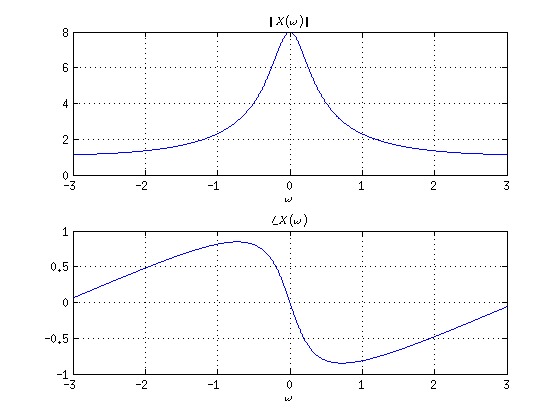
\includegraphics[width=0.6\textwidth]{figs/c4p1c.png}
\label{fig:c4p1c}
\end{figure} 

